\chapter{Tame \& Wild Knots}\label{chap:tame-and-wild-knots}
\def\figdir{figures/wild}
\setlength\epigraphwidth{.7\textwidth}
\epigraph{``And now,'' cried Max, ``let the wild rumpus
  start!''}{---Maurice Sendak, \emph{Where the Wild Things Are}}


The goal of this chapter is to define the basic concepts of
\emph{tameness} and \emph{wildness}. Both of these are defined in
multiple ways throughout the literature, and for the uninitiated, it
can be non-obvious how to reconcile the different characterizations.
We've endeavored to collect some of the most common definitions we've
seen, and show that they are equivalent.\footnote{We will not include
  proofs for \emph{all} of the equivalences, but for the two most
  common definitions, we've included references to full proofs
  whenever we omit the details.} One should note that in general, the
equivalence of these definitions \emph{does not necessarily
  generalize} to higher-dimensional cases, e.g.\ surfaces embedded in
$\RR^4$.

For our ``starting-point'' definitions, we'll use those given in
\cite{Daverman}. These match the definitions used when studying
embeddings of general $m$-manifolds into $n$-manifolds.

Note that beyond this chapter, not much of this material to come will
be called upon explicitly. Nevertheless, we have felt it is important
to include for two reasons:
\begin{enumerate}
  \item Given how ubiquitous the PL category is, we found it
    hard to find references for whether fundamental results like
    ``ambient orientation-preserving homeomorphism guarantees ambient
    isotopy'' are valid in the full Topological category. It appears
    much of this information has become mathematical folklore, which
    can make it difficult for non-experts to approach questions of
    interest about wild knots. We hope this helps to address part of
    that problem.
  \item Second, it provides a good opportunity to ease ourselves into
    thinking about ambient isotopy without immediately rushing to
    Reidemeister's theorem, as this will not be available to us once
    we move into the Topological category.
\end{enumerate}

% we have just sought to centralize this information so the
% reader knows it exists and will not be confused if encountering
% unexpected terms in the literature.\footnote{Finding careful
%   definitions of these terms in the literature can be quite
%   challenging, especially since authors do not always explicitly state
%   which category they are working in. We hope that we have done an
%   adequate job of the compilation.}

\subsection*{Prerequisites \& Further Reading}\label{subsec:further-reading}
Discussing Tame and Wild knots requires some knowledge of PL topology.
We've included a (very) short crash course in
\cref{appendix:pl-topology}, and a more philosophical discussion in
\cref{sec:the-categories}. The former essentially consists of a short
collection of definitions and propositions about affine and convex
sets, ending with the definition of a simplicial complex. If the
reader would like a more detailed reference work, we have some
suggestions.
\begin{itemize}
  \item The standard reference for the topic appears to be
    \cite{Rourke1982}. Although we have not personally used this text,
    it seems to be well-regarded (although we gather that PL topology
    has generally fallen out of favor).
  \item \cite{StarbirdAndSu} offers an excellent
    inquiry-based-learning (IBL) approach accessible to an
    undergraduate. We would highly recommend this text for learning
    the basics of the material; however, as the IBL approach means
    essentially all proofs are left to the reader, those looking for a
    quick-and-easy reference work might consider other sources.
  \item \cite{Bryant2001Jan} gives a very readable birds-eye view
    of PL topology that we found compelling, even though diagrams are
    relatively few and far between.
  \item \cite{Sakai2013} includes comprehensive exposition on
    PL topology through simplicial complexes, without assuming local
    finiteness. We did find the notation and writing style a bit too
    terse for our tastes (especially given the relatively few
    diagrams), but this could be a matter of personal preference.
\end{itemize}
For further reading on the topic of tame/wild embeddings in general,
we found \cite{Daverman} to be an excellent resource with clear
exposition and fantastic illustrations. However, it assumes a high
level of familiarity with prerequisite material, and hence might
inaccessible for most undergraduates.

Anyways, for our first section, we'll give a brief discussion of the
main categories used when studying knots. This is not an area of
expertise for the author, so we would welcome any insights, helpful
examples, or analogies the reader has to offer.

\section{A Word on the Topological, PL, and $C^\infty$
  Categories}\label{sec:the-categories}
First, the philosophical motivation. Wild knots can offer seemingly
pathological behavior. For instance, as we show later in
\cref{ex:fox-artin-curve}, the following arc is impossible to untie:
\begin{figure}[H]
  \centering
  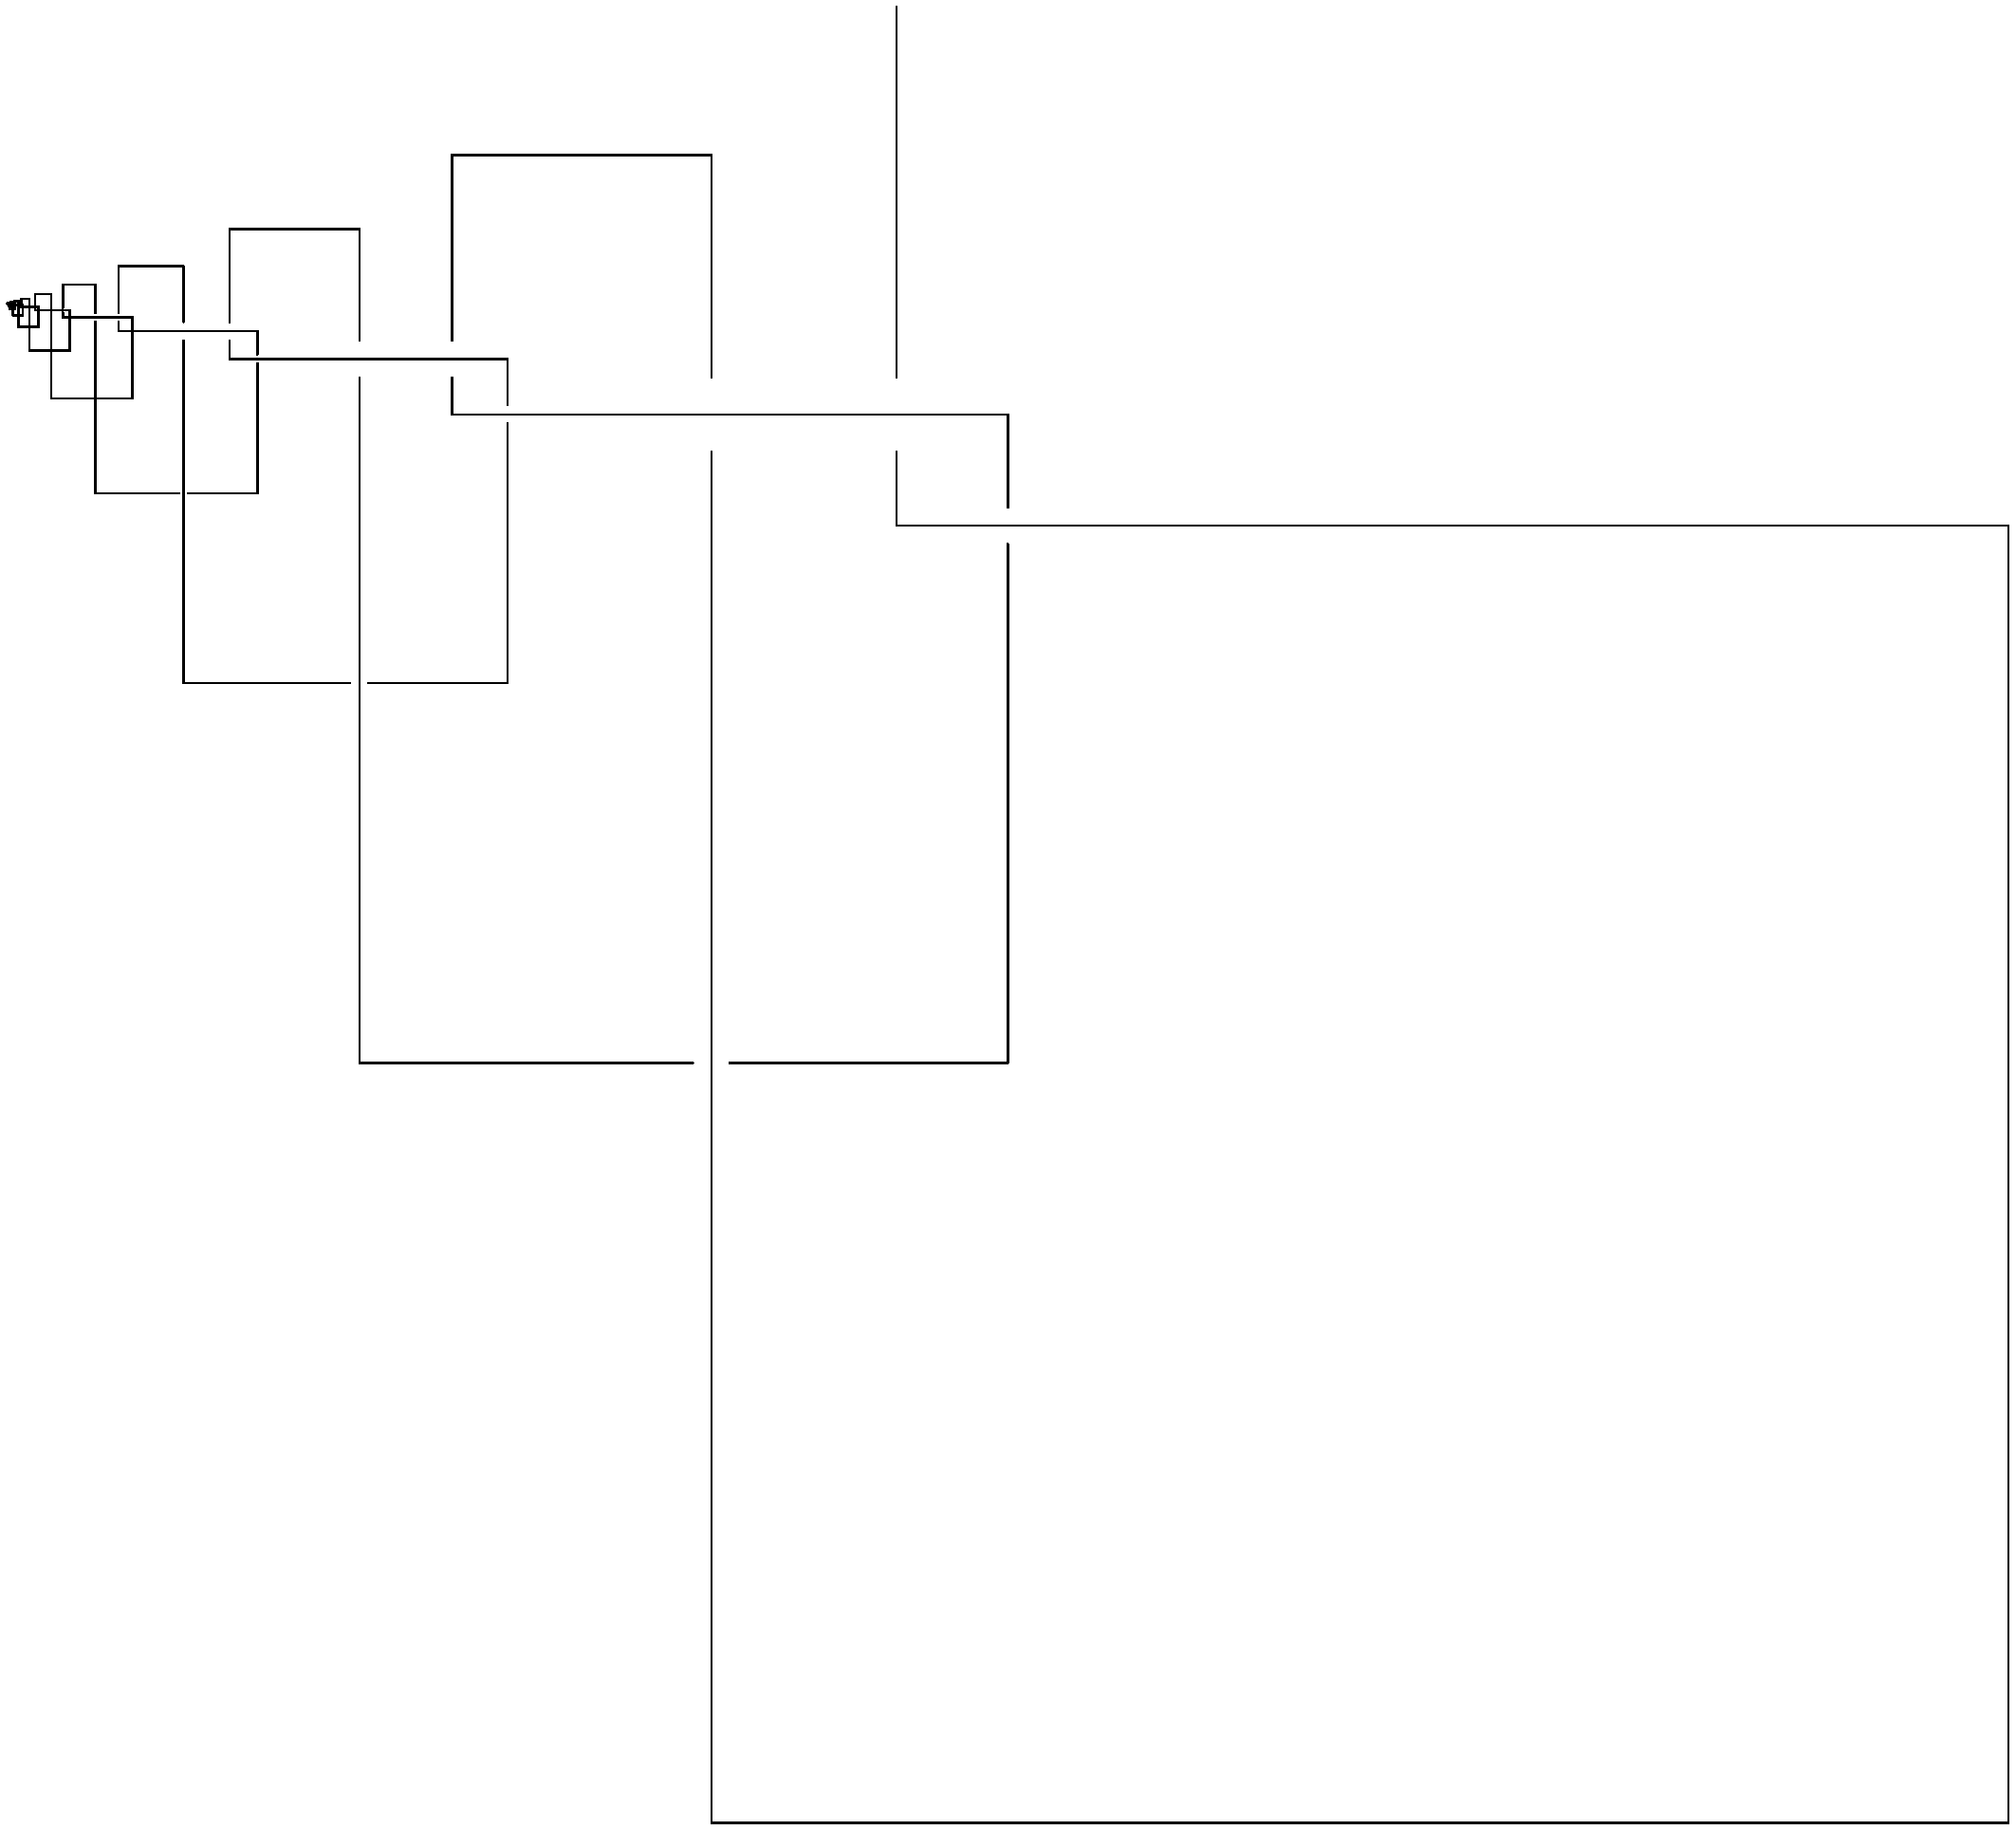
\includegraphics[scale=.2]{\figdir/fox-artin.pdf}
  \caption{A wild arc of \cite{FoxArtin}}
\end{figure}
This counterintuitive property is often listed as one of the reasons
why we omit wild knots from our study of knot theory. Actually, as
we'll show (see \cref{fig:fox-artin-3d-torus} and the associated
discussion), the reason this arc is impossible to unknot is quite
intuitive: If we try to remove each of the stitches in succession,
then at every step we end up dragging some points in the ambient space
\emph{through} the subsequent loop. As we continue to untie, these
same points (together with friends they pick along on the way) get
dragged down further and further towards the wild point, and in the
limit, all of them converge. Hence we lose bijectivity. Not so scary
and mysterious after all!

But in any case: Historically, wild knots have been hard to approach.
Hence knot theory is often restricted to ``nicer'' contexts where
describing the behavior of our knots (and their relationships to each
other) can be reduced to finite, combinatorial means. In the PL
category for instance, we require our knots to decompose into finitely
many linear pieces, and also require any \emph{modifications} we'd
like to make to them to be encoded by maps on the ambient space that
decompose similarly (see \cref{thm:polygonal-ambient-isotopy}). Then,
because linear-flavored objects can be described with finite
information,\footnote{E.g., given the endpoints of a line segment, any
  point $p$ in the middle can be described by a single parameter
  encoding what percentage of the way from end 1 to end 2 $p$ is} this
ends up giving us a context in which essentially \emph{all} of our
questions about knots can be simplified into finite problems (again,
this was the exact idea behind
\cref{part:unknotting-moves-and-combinatorial-representations}).

The point to highlight in the above is that in making a choice of a
particular category to work in, we are requiring both our
\emph{objects} (knots embedded into $\RR^3$) and our \emph{morphisms}
(functions deforming $\RR^3$) to have a particular kind of structure.
By choosing our restrictions judiciously, we can strike a nice balance
between generality and tidiness in the theories we construct.

As seen through the existence of wild knots in the Topological
category, working in different categories can yield very different
results in the theory. Hence it is important for us to always clarify
exactly which category we're assuming, so that readers have a sense
for the scope of our results. The goal of this section is to remind us
of this fact, and of some basic properties of each of the common
categories, which we list below.

% \subsection{The Categories}
% The most common categories for working with knots are as follows:
\begin{itemize}
  \item The \emph{Topological} category.
    \begin{itemize}
      \item Objects: Embeddings $K : S^1 \into \RR^3$ (or $S^3$)
      \item Morphisms: Ambient isotopies $F : [0,1] \times \RR^3 \to
        \RR^3$.\footnote{Equivalently, ambient orientation-preserving
        homeomorphisms (see \hyperlink{link:equiv-in-top}{6.3.2})}
      \item Notes: Most general context to work in, but allows
        ``pathological'' behavior.
    \end{itemize}
  \item The \emph{PL} category.
    \begin{itemize}
      \item Objects: PL Embeddings $K : S^1 \into \RR^3$
      \item Morphisms: PL Ambient isotopies $F : [0,1] \times \RR^3
        \to \RR^3$.\footnote{Equivalently, ambient
        orientation-preserving PL homeomorphisms (see
        \hyperlink{link:equiv-in-pl}{6.3.2})}
      \item Notes: Rarely worked with directly, but forms the backbone
        of almost all modern combinatorial knot theory. Underpins
        Reidemeister's theorem.
    \end{itemize}
  \item The $C^k$ category ($k \geq 1$).
    \begin{itemize}
      \item Objects: $k$-times continuously differentiable embeddings
        $K : S^1 \into \RR^3$.
      \item Morphisms: $k$-times continuously differentiable ambient
        isotopies $F : [0,1] \times \RR^3 \to
        \RR^3$.
      \item Notes: Uncommon. By \cref{thm:c1-suffices} in
        \cref{chap:feral-gallery} (together with an argument that
        every tame knot can be realized by a $C^1$ representative),
        this is more-or-less isomorphic to the PL Category. However it
        does allow for knots whose diagrams in $\RR^2$ are
        \emph{feral} (see \cref{sec:feral-points}).
    \end{itemize}
  \item The $C^\infty$ category, also commonly referred to as the
    \emph{Smooth} category (although we \emph{vehemently} protest this
    choice of phrasing, since we've found authors are not always
    consistent on whether ``smooth'' means ``$C^1$'' or
    ``$C^\infty$,'' especially between fields).
    \begin{itemize}
      \item Objects: Infinitely-differentiable embeddings $K : S^1
        \into \RR^3$.
      \item Morphisms: Infinitely-differentiable ambient isotopies $F
        : [0,1] \times \RR^3 \to \RR^3$.
      \item Notes: Also known to be ``equivalent'' to the PL category
        (in the sense that every $C^\infty$ knot is topologically
        ambient-isotopic to a PL knot, and vice versa).
    \end{itemize}
\end{itemize}
% Since the vast majority of knot theory assumes the PL category, we'll
% discuss its correspondence with polygonal knots very briefly.

% \subsection{PL $==$ Polygonal}

% {\color{blue}\huge We show that PL embeddings consist of finite unions
%   of polygonal segments. }

With these distinctions in mind, we now move into a discussion of
various \emph{tameness} properties, which essentially describe whether
an embedding can be encoded by a PL one.

\section{What it Means to be Tame, Wild, and (Locally)
  Flat}\label{sec:tame-wild-definitions}
We'll begin by clarifying some vocabulary that caused us some
confusion in trying to understand the characterization of tame vs.\
wild knots. As discussed in the preface, there are many definitions
given for tameness.\footnote{We reproduce these below, but if the
  reader would like to see them in their original context, they were
  Common Definitions \hyperlink{def:cdef1}{1}-\hyperlink{def:cdef4}{4}
  in the Preface.} The examples we gave were the following:
\begin{leftbar}\vspace{-.3725cm}
  \setcounter{commondefx}{0}
  \begin{commondef}\label{def:cdef1b}
    We say a knot $K : S^1 \into \RR^3$ is \emph{tame} iff it is
    ambient isotopic to a polygonal knot.
  \end{commondef}
  \begin{commondef}\label{def:cdef2b}
    We say a knot $K : S^1 \into \RR^3$ is \emph{tame} iff for every
    point $x$ on $K$, there exists a neighborhood $U_x$ such that the
    pair $(U_x, K \cap U_x) \cong $ the standard $(\mrm{ball},
    \mrm{diameter})$ pair.
  \end{commondef}
  \begin{commondef}\label{def:cdef3b}
    We say a knot $K : S^1 \into \RR^3$ is \emph{tame} iff it can be
    thickened to an embedding of a solid torus.
  \end{commondef}
  \begin{commondef}\label{def:cdef4b}
    We say a knot $K : S^1 \into \RR^3$ is \emph{tame} iff it has a
    diagram with finitely many crossings.
  \end{commondef}
\end{leftbar}
Of these, \cref{def:cdef1b} is the closest to the definition given in
\cite{Daverman} for tameness in the context of embeddings of general
manifolds. \cref{def:cdef2b} corresponds to the definition of
\emph{local flatness}, but that turns out to coincide with tameness in
the case of embeddings $S^1 \into \RR^3$. With some added
clarification on what ``thickened'' means in \cref{def:cdef3b}, we
were able to find a convincing argument for the $(\implies)$
direction, but have not been able to find a similar one for the
$(\impliedby)$ direction. Finally, we believe \cref{def:cdef4b} is
misleading, and hence should be avoided.

\subsection{Basic Definition}
Almost all of our definitions will match those given in the
introduction in \cite{Daverman}. Note, they define \emph{equivalence
  of embeddings} in terms of ambient homeomorphisms, not ambient
isotopies. In \cref{sec:corr-cdef-1}, we show that as far as tameness
vs.\ wildness is concerned, ``ambient homeomorphism'' can be replaced
by ``ambient orientation-preserving homeomorphism'' in the above, at
which point the correspondence with ambient isotopy can be shown. We
provide references for proofs in each of the Topological, PL, and
$C^1$ categories.

% Also note that \cref{def:ambient-homeomorphic} does not require an
% \emph{orientation-preserving} homeomorphism; this done so as to be
% consistent with \cite{Daverman}. However, as we'll show in
% \cref{sec:orientation}, choosing orientation-preserving homeomorphisms
% in $\RR^n$ yields the exact same theory of tameness/wildness/flatness
% that we would have if we only required homeomorphism.
\begin{definition}[Ambient
  homeomorphic]\label{def:ambient-homeomorphic}
  Let $(X, \ms T)$, $(Y, \ms S)$ be topological spaces. Let $\iota_0,
  \iota_1 : X \into Y$ be embeddings.\footnote{Recall, this just means
    $\iota_0, \iota_1$ are homeomorphisms onto their images.} Then
  $\iota_0$, $\iota_1$ are said to be \emph{ambient homeomorphic} if
  there exists a homeomorphism $f : Y \to Y$ such that $f \circ
  \iota_0 = \iota_1$.
\end{definition}
Note, taking $t=1$ in the definition of ambient isotopy directly
implies the existence of an ambient homeomorphism. It is the converse
we are uncertain about (although we expect it to be true).
% {\color{blue} Need to add definition of a PL manifold to the appendix}
\begin{definition}[Tame \& Wild Embeddings]\label{def:tame-and-wild}
  Let $X$ be a polyhedron and let $Y$ be a PL manifold. Then we say $K
  : X \into Y$ is a \emph{tame embedding} iff it is ambient
  homeomorphic to a PL embedding. An embedding that is \emph{not} tame
  is called \emph{wild}.
\end{definition}
This is slightly different from the definition of tame \& wild
\emph{subsets}, which we alert the reader to now:
\begin{definition}[Tame \& Wild Subsets]\label{def:tame-and-wild-subsets}
  Let $Y$ be a PL manifold, and let $A \subseteq Y$ be closed. Then
  $A$ is said to be \emph{tame} iff there exists an ambient
  homeomorphism $f : Y \to Y$ such that $f(A)$ is a subpolyhedron of
  $Y$. $A$ is said to be \emph{wild} if it is ambient homeomorphic to
  a simplicial complex but not tame.
\end{definition}
The correspondence can be established through the following
proposition, which is stated informally in \cite{Daverman}.
\begin{proposition}\label{prop:tame-and-wild-subset-embedding-correspondence}
  Let $Y$ be a PL manifold and let $A \subseteq Y$ be closed. Use
  $\iota$ to denote the inclusion $\iota : A \into Y$. Then $A$ is
  \emph{tame as a subset} iff there exists a polyhedron $X$ and a
  homeomorphism $f : X \to A$ such that $\iota \circ f : X \to Y$ is a
  tame embedding.
\end{proposition}
Lastly, we describe two local properties embeddings can have:
\emph{local flatness}, and \emph{local tameness}.
\begin{definition}[Local Flatness at a Point]\label{def:locally-flat}
  Let $X$, $Y$ be $m$ and $n$-manifolds respectively, with $m < n$.
  Let $K : X \into Y$ be an embedding, and let $x \in X$. Then we say
  $K$ is \emph{locally flat} at $x$ iff there exists an open set
  $U_{x} \in Y \st K(x) \in U_x$ and there exists a homeomorphism $f :
  U_x \to \RR^n$ such that $\fim{f}{U_x \cap K(X)} =
  \RR^m$.\footnote{Long way of saying $(U_x, U_x \cap K(X)) \cong
    (\RR^n, \RR^m)$. We just chose the former to avoid having to
    introduce new notation.}
\end{definition}
Note, with all variables as above, sometimes we'll also say $f$ is
\emph{locally flat} at $f(x)$.
\begin{definition}[Local Flatness of an Embedding]
  With all variables quantified as above, then if $K$ is locally flat
  for all $x \in X$, then we call $K$ \emph{locally flat}.
\end{definition}
Note, the definition of local flatness is just encoding the idea that
we can ``straighten out'' our embedded copy of $X$ in $Y$ around each
point in the image. We can define \emph{local tameness} in a similar
manner.
\begin{definition}[Local Tameness of an Embedding]\label{def:locally-tame}
  Let $X$ be a polyhedron with a fixed triangulation, and let $N$ be a
  \emph{topological} $n$-manifold. Let $K : X \into N$ be an
  embedding. Then $K$ is said to be \emph{locally tame} iff for every
  $x \in X$, there exists \np{a PL neighborhood $U_x \subseteq N \st
    K(x) \in U_x$} and a homeomorphism $f_x : U_x \to \RR^n$ such that
  \[
    f_x \circ K\vert_{\fpre{K}{U_x}}
  \]
  is PL with respect to the above fixed triangulation of $X$.
\end{definition}
Of course, for our purposes today we'll primarily be interested in the
case of embeddings $K : S^1 \into \RR^3$. Can the definitions above be
made to match Common Definitions
\hyperlink{def:cdef1b}{1}-\hyperlink{def:cdef:4b}{4} in these cases?
The following gives the affirmative for \hyperlink{def:cdef1b}{1} and
\hyperlink{def:cdef:4b}{2}, but we will need to wait until later to
determine the answer for \hyperlink{def:cdf3b}{3} and
\hyperlink{def:cdf3b}{4}.

\section{Correspondence with Common Def.\ 1}\label{sec:corr-cdef-1}
There are two main sticking points in establishing the correspondence
here. First, can replace ``homeomorphism'' with
``orientation-preserving homeomorphism'' in our definitions for
tameness / wildness / local flatness and get the same theory? And
second, is the existence of an orientation-preserving homeomorphism
equivalent to the existence of an ambient isotopy? We show the
affirmative for the former in $\RR^n$, and direct the reader to
existing proofs for the latter in $\RR^3$.

\subsection{Homeomorphism vs.\ Orientation-Preserving Homeomorphism}
Showing the equivalence of ``homeomorphism'' and
``orientation-preserving homeomorphism'' in $\RR^n$ is
straightforward. In each of the PL, $C^1$, and Topological categories,
every homeomorphism must be either orientation-preserving or
orientation-reversing, hence we can make a non-orientation-preserving
homeomorphism into an orientation-preserving one by simply applying a
flip as necessary.
\begin{theorem}\label{thm:orientation-preserving-or-not}
  Every homeomorphism $f : \RR^n \to \RR^n$ is either
  \emph{orientation-preserving} or \emph{orientation-reversing}.
\end{theorem}
\begin{sproof}[Sketches]
  We give a sketch for a proof in each category.
  \begin{itemize}
    \item (PL) Given a fixed triangulation $K$ of $\RR^n$ and an
      $n$-simplex $\triangle^n \in K$, note that any PL homeomorphsim
      either fixes or reverses the orientation of $\triangle^n$. Now,
      the orientation of $\triangle^n$ induces a canonical orientation
      on each of its $(n-1)$-faces $\triangle^{n-1}$. This gives us a
      unique compatible orientation on each of the other simplices
      ${\triangle^{n'}} $ that have $\triangle^{n-1}$ as a face. One
      can then show this extends to a unique compatible orientation
      for all of $K$.
    \item ($C^1$)\footnote{See
      \url{http://www.math.columbia.edu/~faulk/Lecture6.pdf} for
      a bit more detail.} Observe that in the $C^1$ category, the
      derivative matrix
      \[
      Df(x) =
      \begin{bNiceMatrix}
        \pd{f_1}{x_1}(x) & \pd{f_1}{x_2}(x) & \Cdots & \pd{f_1}{x_n}(x) \\[.5em]
        \pd{f_2}{x_1}(x) & \pd{f_2}{x_2}(x) & \Cdots & \pd{f_2}{x_n}(x) \\[.5em]
        \Vdots & \Vdots & \Ddots & \Vdots \\
        \pd{f_n}{x_1}(x) & \pd{f_n}{x_2}(x) & \Cdots & \pd{f_n}{x_n}(x)
      \end{bNiceMatrix}
      \]
      exists, is continuous in $x \in \RR^n$, and invertible
      everywhere ($f$ is $C^1$ with $C^1$ inverse). Now, note that
      for all $x \in \RR^n$, the local orientation of $\fim{f}{\RR^n}$ is
      given by $\sgn(\det(Df(x)))$. One can show that $\det(Df(x))$ is
      continuous in $x$. Now, observe that $\RR^n$ is path-connected
      (hence $\fim{f}{\RR^n}$ is as well), and consider an arbitrary path
      $\gamma : [0,1] \into \RR^n$. Observe that $\det(Df(\gamma(t)))
      \neq 0$ for all $t$ ($Df(x)$ is invertible everywhere), hence by
      continuity, the sign of $Df(x)$ is the same at the endpoints
      $\gamma(0)$, $\gamma(1)$. Since $\gamma$ was arbitrarily chosen,
      it follows that $\sgn(Df(x))$ is constant over $\RR^n$. Hence we
      get a unique orientation over all of $\fim{f}{\RR^n}$.
    \item (Topological) This is given in \cite{Crowell1963} on pg.\ 8,
      although the matter is essentially definitional. We've
      reproduced a slightly more detailed version below for
      completeness.

      First, we consider homeomorphisms of $S^n$. Let $g : S^n \to
      S^n$ be a homeomorphism. Observe that the induced map $g_* :
      H_n(S^n) \to H_n(S^n)$ is an isomorphism. Since $H_n(S^n) =
      \ZZ$, there are only two choices for $g_*$, determined by
      whether $g_*(1) = 1$ or $g_*(1) = -1$. In the first case, we
      call $g$ \emph{orientation-preserving}, and in the second,
      \emph{orientation-reversing}.

      Recall that we can think of $S^n$ as a one-point
      compactification of $\RR^n$ by $S^n \cong \RR^n \cup
      \set{\infty}$. Observe that in this light, our original
      homeomorphism $f : \RR^n \to \RR^n$ has a unique extension to
      $\ms f : \RR^n \cup \set{\infty} \to \RR^n \cup \set{\infty}$ by
      taking
      \[
      \ms f(x) =
      \begin{cases}
        f(x) & x \in \RR^n \\
        \infty & x = \infty.
      \end{cases}
      \]
      hence $f$ is either orientation-reversing or
      orientation-preserving.

      Again, this is essentially definitional. The harder part is show
      that this is consistent with both of the definitions above. We
      won't do that.\renewcommand{\qed}{\hfill $\square$}\qedhere
  \end{itemize}
\end{sproof}
As a simple corollary we have the desired equivalence of
``homeomorphism'' and ``orientation-preserving homeomorphism'' in the
definitions of tameness, wildness, and locally flat.
\begin{corollary}
  An embedding $K : X \into \RR^n$ is tame iff there exists an
  orientation-preserving ambient homeomorphism $f : \RR^n \to \RR^n$
  such that $f \circ K$ is a PL embedding. Analogously for local
  flatness.
\end{corollary}
\begin{sproof}~
  \begin{iffproof}
  \item Suppose we have an orientation-preserving ambient
    homeomorphism satisfying the desired properties. Then take this to
    be our ambient homeomorphism and we're done.
  \item Suppose we have a homeomorphism satisfying the desired
    properties. If it's orientation-preserving, then we're done. If
    is not, then by \cref{thm:orientation-preserving-or-not}, it is
    orientation-reversing. Hence, compose it with
    \[
      g =
      \bk{
        \hspace{.7em}
        \begin{NiceArray}{CCCCC}
          \hspace{-.7em}-1 & 0 & 0 & \Cdots & 0 \\
          0 & 1 & 0 & \Cdots & 0 \\
          0 & 0 & 1 & \Cdots & 0 \\
          \Vdots & \Vdots & \Vdots & \Ddots & \Vdots \\
          0 & 0 & 0 & \Cdots & 1
        \end{NiceArray}
      }.
    \]
    And observe that the result is an orientation-preserving
    homeomorphism, and that we can take a subdivision of our
    triangulation on $\RR^n$ to show that we get a PL embedding, as
    desired. \qedhere
  \end{iffproof}
\end{sproof}
Hence, as far as tameness, wildness, and local flatness are concerned,
``homeomorphism'' and ``orientation-preserving homeomorphism'' are
equivalent.

\subsection{Orientation-Preserving Homeomorphism vs.\ Ambient Isotopy}
Now, we collect some references establishing the equivalence of
orientation-preserving homeomorphism and ambient isotopy in each of
the three categories.

\begin{enumerate}
  \item \emph{The Topological Category:} Here, the desired result is
    provided by \cite{Fisher} in Theorem 4.\hypertarget{link:equiv-in-top}{}
    \begin{leftbar}
      \begin{definition}[Deformation (Fisher)]
        A \emph{deformation} of a manifold $M$ is a homeomorphism $f :
        M \to M$ such that $f$ is isotopic to the identity.
      \end{definition}
      \begin{theorem}[Fisher, Theorem 4]
        If $X = M$ is an $n$-manifold, then every $f$ in the group
        $G^0(M)$ of homeomorphisms of $M$ is a deformation of $M$.
      \end{theorem}
    \end{leftbar}
  \item \emph{The PL Category:} One can find the desired proof in
    \cite{burde2003knots}. The numbering below follows that of the
    second edition.\hypertarget{link:equiv-in-pl}{}
    \begin{leftbar}
      \begin{theorem}[Burde \& Zieschang, Proposition 1.10]
        Let $\msf K_0$, $\msf K_1 : S^1\into S^3$ be PL. Then there
        exists a PL orientation-preserving homeomorphism $f : S^3 \to
        S^3$ such that $f\circ \msf K_0 = \msf K_1$ iff there exists a
        PL ambient isotopy taking $\msf K_0$ to $\msf K_1$.
      \end{theorem}
      \begin{corollary}[Burde \& Zieschang, Corollary 3.16]
        If two tame knots are topologically equivalent\footnote{I.e.,
          by topological ambient isotopy / toplogical
          orientation-preserving homeomorphism} then they are PL
        equivalent.
      \end{corollary}
    \end{leftbar}
  \item \emph{The $C^1$ Category:} A proof of the following is
    provided in \cite{milnor1997topology} as Lemma 2 in \S 6 (pg.\
    34).
    \begin{leftbar}
      \begin{lemma}[Milnor, Lemma 2]
        Any orientation-preserving diffeomorphism $f$ of $\RR^m$ is
        $C^1$ isotopic to the identity.
      \end{lemma}
    \end{leftbar}
\end{enumerate}
We also collect two helpful online threads the reader can investigate
if interested.
\begin{itemize}
  \item See \cite{MO-equiv}'s post on MathOverflow for a general
    discussion of references for proofs in each category.
  \item See \cite{SE-equiv}'s post on StackExchange for a proof of the
    PL case. Note, user
    \cite{WhippedCream}'s post in the same thread includes the
    argument for the $C^1$ category given in
    \cite{milnor1997topology} with a few more details filled in.
\end{itemize}
In any case, we have our desired result:
\begin{corollary}\label{cor:equivalence-of-cdef1}
  Let $K : S^1 \into \RR^3$. Then $K$ is ambient homeomorphic to a PL
  knot iff $K$ is ambient isotopic to a PL knot. In particular,
  \cref{def:tame-and-wild} and Common Definition
  \hyperlink{def:cdef1b}{1} are equivalent.
\end{corollary}


\section{Correspondence with Common Def.\ 2}\label{sec:corr-cdef-2}
In the following, we examine the correspondence between
\cref{def:tame-and-wild} and Common Definition
\hyperlink{def:cdef2b}{2} (this was ``tame'' iff ``locally flat''). We
prove that for embeddings $K : S^1 \into \RR^3$, ``tame implies
locally flat.'' We outsource most of the ``locally flat implies tame''
proof to \cite{Bing}. Because the ``tame implies locally flat''
argument is somewhat trivial, we'll spice it up a bit by using the
opportunity to demonstrate a technique for explicitly constructing
ambient isotopies.

Because it is generally \emph{not} true that tameness is equivalent to
local flatness for arbitrary embeddings of $m$-manifolds in
$n$-manifolds, we would like to discourage the use of Common
Definition \hyperlink{def:cdef2b}{2} as the ``starting-point''
definition of tameness in knot theory. A few more notes, which we
summarize from \cite{Daverman}:
\begin{itemize}
  \item It is true that in general, if $M$, $N$ are PL $m$, $n$
    manifolds with $M$ tamely embedded in $N$, then if $n - m \neq 2$,
    $M$ is locally flat in $N$. (\cite{Daverman}, Theorem 1.2.1)
  \item With all variables as above, in the case $n - m = 2$, $M$
    \emph{is} locally flat at a dense set of points.
  \item Local flatness generally does not imply tameness.
\end{itemize}

With these facts in mind, we move on to establishing that tameness and
local flatness \emph{do} coincide in the case of $S^1 \into \RR^3$.
First, we note that the definition for local flatness
(\cref{def:locally-flat}) can be reworded slightly. The claim is
trivial; we are including for the sake of being very explicit.
\begin{lemma}\label{lem:equivalent-locally-flat-def}
  The $(U_x, U_x \cap K(X)) \xmapsto{f} (\RR^n, \RR^m)$ condition in
  the definition of local flatness can be replaced with $(U_x, U_x
  \cap K(X)) \xmapsto{f} (\text{$n$-ball, sub-$m$-ball})$ where
  $\partial \pn{\text{sub-$m$-ball}} \subseteq \partial
  \pn{\text{$n$-ball}}$.
\end{lemma}
\begin{sproof}
  Follows directly from the fact that $n$-ball's are homeomorphic to
  $\RR^n$.
\end{sproof}
We'll often use this definition above when discussing local flatness.
\begin{lemma}\label{lem:local-flatness-homeomorphism}
  Let $K_0, K_1 : S^1\into \RR^3$. Suppose there exists a
  homeomorphism $f : \RR^3 \to \RR^3$ such that $f \circ K_0 = K_1$.
  Then $K_0$ is locally flat iff $K_1$ is.
\end{lemma}
\begin{sproof}~
  \begin{iffproof}
  \item Suppose $K_1$ is locally flat. The proof that $K_0$ is as well
    is essentially identical to the one below.
  \item Suppose $K_0$ is locally flat. We want to show $K_1$ is. To
    that end, let $p \in \fim{K_1}{S^1}$. Then $f^{-1}(p) \in
    \fim{K_0}{S^1}$. Define $q = f^{-1}(p)$.

    Since $K_0$ is locally, flat there exists an open set $U_{q}
    \subseteq \RR^3$ and a homeomorphism $f_q : \RR^3 \to \RR^3$ such
    that
    \begin{enumerate}
      \item $q \in U_q$, and
      \item $(U_q, \fim{K_0}{S^1} \cap U_q) \xmapsto{f_q}
        (\text{3-ball, 3-ball diameter})$.
    \end{enumerate}
    Define $U_p = \fim{f}{U_q}$, and note that $U_p$ is open with $p
    \in U_p$. Now, observe that $f_p : \RR^3 \to \RR^3$ defined by
    \[
      f_p = f_q \circ f^{-1}
    \]
    is a homeomorphism satisfying
    \[
      (U_p, \overleftarrow{K_1}(S^1) \cap U_p) \xmapsto{f_p}
      (\text{3-ball, 3-ball diameter}).
    \]
    Hence $K_1$ is locally flat at $p$. Since $p$ was arbitrarily
    chosen, it follows that $K_1$ is locally flat. \qedhere
  \end{iffproof}
\end{sproof}
We use this in the following proposition, which is given as an
exercise in \cite{Daverman}.
\begin{proposition}[Daverman and Venema, Exercise
  1.2.3]\label{prop:tame-implies-locally-flat}
  Every tame $1$-sphere in $\RR^3$ is locally flat.
\end{proposition}
Before we give the proof, an important note:
\begin{note}
  The argument below is \emph{comically} overkill, but we've included
  it because the general technique of ``parameterizing a closed region
  by lines connecting \np{points on the boundary} to \np{points on
    some 1-manifold we want to deform}'' is what underpins a lot of
  our ambient isotopy proofs later.\footnote{E.g., this appears in the
    proof of \cref{prop:replacing-by-same-endpoints} when we make
    reference to \cref{prop:pt-to-barycenter}.} The idea is that we
  can take the boundary to be fixed, after which \emph{all} of the
  interior points must ``follow'' the points on the 1-manifold we're
  deforming.

  Because the explicit construction required for this technique is
  often so tedious, we will usually choose to omit it in our proofs
  and speak in only vague terms instead. This might make it a
  challenge for the reader to fill in the gaps on their own, so we've
  chosen to showcase the technique in detail here to expose the key
  ideas in a more approachable context. Hopefully this will help with
  the readability the proofs to come.
\end{note}
\begin{sproof}
  By \cref{lem:local-flatness-homeomorphism}, it suffices to show
  polygonal knots are locally flat. Hence, let $\msf K : S^1 \into
  \RR^3$ be polygonal, and let $x \in \fim{\msf K}{S^1}$. Also let $E$
  denote the set of all straight edges in $\fim{\msf K}{S^1}$; by
  definition, $E$ is finite. We proceed with two subcases.
  \begin{enumerate}[label=\arabic*)]
    \item Suppose $x$ is an interior point of some $\msf E_x \in E$
      (i.e., $x$ is not a vertex). Then let
      \[
      \varepsilon = \min_{\substack{\msf E \in E \\ \msf E \neq \msf
      E_x}} d(x, \msf E),
      \]
      and observe $\varepsilon > 0$. Then $(B_\varepsilon(x),
      B_\varepsilon(x) \cap \msf{K})$ is trivially homeomorphic to the
      $(\text{3-ball, 3-ball diameter})$ pair.
    \item Now, suppose $x$ is one of the vertices of $\msf K$ (i.e.,
      one of the points where we join two polygonal segments). We
      construct the desired ambient homeomorphism explicitly.

      Let $\msf E_{x,1}, \msf E_{x,2} \in E$ be the distinct edges
      with $\msf E_{x,1} \cap \msf E_{x,2}= \set{x}$. Let
      \[
      \varepsilon = \frac{1}{2} \min_{\substack{\msf E \in E \\ \msf E
      \neq \msf E_{x,1} \\ \msf E \neq \msf E_{x, 2}}} d(x, \msf E),
      \]
      and observe $\varepsilon > 0$. Note that since the other
      endpoints of $\msf E_{x,1}$, $\msf E_{x,2}$ correspond to the
      start of new strands, $\varepsilon <
      \frac{1}{2}\mrm{length}(\msf E_{x,1})$,
      $\frac{1}{2}\mrm{length}(\msf E_{x,2})$. We draw a diagram in
      the plane of $\msf E_{x,1}$, $\msf E_{x,2}$ below.
      \begin{figure}[H]
        \centering
        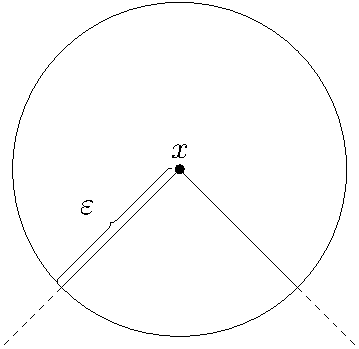
\includegraphics[scale=.75]{\figdir/polygonal-vertex-ball.pdf}
        \caption{$x$, shown together with a 2D cross section of the
          closed ball $\ol{B_\varepsilon(x)}$ and the two line
          segments $\msf E_{x,1}$, $\msf E_{x,2}$}
      \end{figure}
      Note that $\msf E_{x,1}$, $\msf E_{x,2}$ partition this
      cross-section of $B_\varepsilon(x)$ into two regions $R_1$,
      $R_2$, each bounded by $\msf E_{x,1} \cup \msf E_{x,2}$ a
      circular arc (which we'll call $A_1, A_2$ respectively).
      \begin{figure}[H]
        \centering
        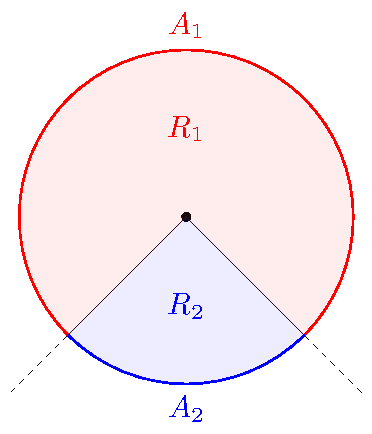
\includegraphics[scale=.75]{\figdir/polygonal-vertex-ball-labeled.pdf}
        \caption{The diagram with $R_1, R_2$, $A_1, A_2$ labeled.}
      \end{figure}
      By some trig, one can find explicit parameterizations of lines
      linking each point of $A_1$ to a point of $A_2$ such that none
      of the lines cross.
      \begin{figure}[H]
        \centering
        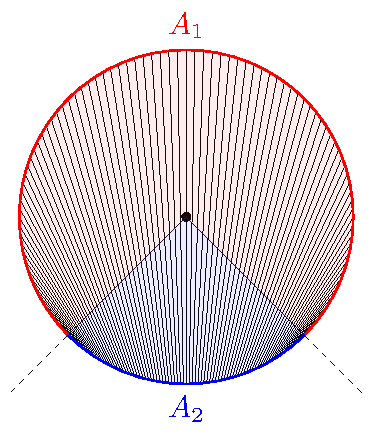
\includegraphics{\figdir/polygonal-vertex-ball-lines.pdf}
        \caption{An example of the lines}
      \end{figure}
      Note that each of these lines intersect $\msf E_{x,1} \cup \msf
      E_{x,2}$ at a unique point. Using this, we can parameterize
      every point $p$ in the region $R_1^\circ$ as follows (and
      analogously for each $q \in R_2^\circ$):
      \begin{enumerate}
        \item Let $\ell_p$ be the unique line through $p$ (guaranteed
          uniqueness since none of the lines cross).
        \item Let $c_p$ be the unique point of $A_1 \cap \ell_p$, and
          let $e_p$ be the unique point of $(\msf E_{x, 1} \cup \msf
          E_{x,2}) \cap \ell_p$. Then observe that there exists a
          unique $\lambda \in [0,1]$ such
          that\footnote{\label{foot:is-just-convex-comb}Note, we're
          really just writing $p$ as a convex combination of $c_p$ and
          $e_p$.}
          \[
          p = \lambda c_p + (1 - \lambda) e_p.
          \]
      \end{enumerate}
      \begin{figure}[H]
        \centering
        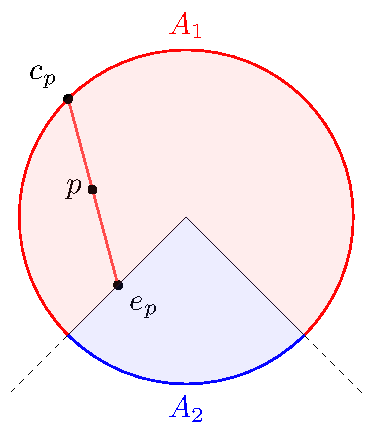
\includegraphics[scale=.75]{\figdir/polygonal-vertex-ball-single-pt-lines.pdf}
        \caption{An example of $c_p, e_p$, with $\ell_p$ shown in red}
      \end{figure}
      This gives us lines like the following:
      \begin{figure}[H]
        \centering
        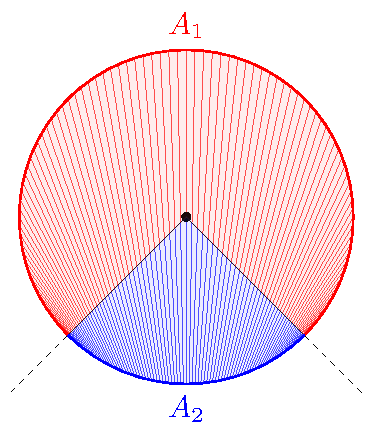
\includegraphics[scale=.75]{\figdir/polygonal-vertex-ball-lines-colored.pdf}
        \caption{The lines after being split over $\msf E_{x,1} \cup
          \msf E_{x,2}$}\label{fig:colored-split}
      \end{figure}
      Now, observe that if we fix ${\color{red}A_1} \cup {\color{blue}
      A_2}$, then the position of any point in $B_\varepsilon(x) \cap
      \aff\pn{\msf E_{x,1} \cup \msf E_{x,2}}$ is fully determined
      by the position of the corresponding $e_p$.\footnote{The $\aff$
      here is just used to restrict $B_\varepsilon(x)$ to the $\msf
      E_{x,1} \cup \msf E_{x,2}$ plane.}

      One can perform a similar parameterization to make each of the
      $e_p$'s themselves depend only on the position of our vertex $x$
      (in this case, the two points of $\ol{B_\varepsilon(x)} \cap
      \pn{\msf E_{x,1} \cup \msf E_{x,2}}$ play the role of the
      $c_p$'s, and $x$ plays the role of the $e_p$'s). Together with
      the above, this makes the position of \emph{every} point in
      $B_\varepsilon(x) \cap \aff\pn{\msf E_{x,1} \cup \msf E_{x,2}}$
      dependent only on the position of $x$.

      Finally, we extend this to all of $B_\varepsilon$. There are two
      ways to do this. One is to ``rotate'' around the axis passing
      through the midpoints of ${\color{red} A_1}$ and ${\color{blue}
      A_2}$, applying the same parameterization in each of the rotated
      sections. This gives us a cone-shaped blue region in $3$D, and
      the complementary-shaped red region. The second is as follows:
      LOG, suppose that $\aff\pn{\msf E_{x,1} \cup \msf E_{x,2}}$ is
      parallel to the $xy$ plane. Then ``extend'' the lines in the $z$
      direction by performing an identical parameterization to the
      above in each parallel cross section. Note, as we go further
      up/down in $z$, the $c_p$ get closer to $x$.

      \begin{figure}[H]
        \centering
        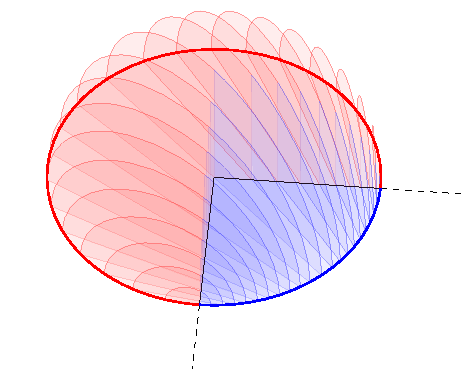
\includegraphics[scale=1.125]{\figdir/polygonal-vertex-ball-lines-colored-3d.pdf}
        \caption[Lines extended to planes]{The $z>0$ portion of the
          sets defined by ``extending'' our lines in the $z$ direction
          within $B_\varepsilon(x)$.}
      \end{figure}
      \begin{figure}[H]
        \centering
        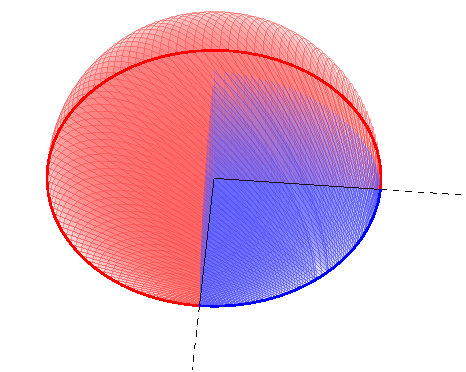
\includegraphics[scale=.75]{\figdir/polygonal-vertex-ball-lines-colored-3d-dense.pdf}
        \caption{A denser version of the same plot.}
      \end{figure}
      Now, consider the map that takes $x$ to the midpoint of the
      secant line between the ends of $\msf E_{x,1}$, $\msf E_{x,2}$,
      with all the other points in $B_\varepsilon(x)$ following $x$ by
      way of their parameterizations.\footnote{Note, we can turn this
      into an ambient isotopy directly by sliding our points along
      these lines.}
      \begin{figure}[H]
        \centering
        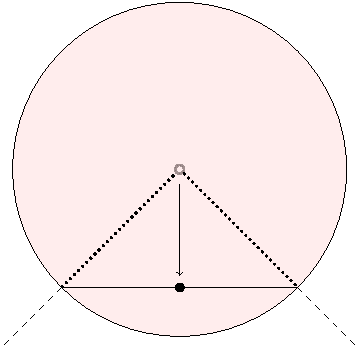
\includegraphics[scale=.75]{\figdir/polygonal-vertex-ball-lines-secant.pdf}
        \caption{Taking $x$ to the secant line}
      \end{figure}
      One can verify that this yields a homeomorphism (in fact, a PL
      homeomorphism) on $\ol{B_\varepsilon(x)}$ fixing the boundary.
      At last, one can take an open sub-ball around the shifted $x$
      and show that it yields a $(\text{3-ball, 3-ball diameter})$
      pair, as desired.
  \end{enumerate}
  In either case, we see $\msf K$ is locally flat at $x$. By
  \cref{lem:local-flatness-homeomorphism}, it follows that any tame
  knot is locally flat.
\end{sproof}
Again, the proof is overkill. The point is just that one should think
of this technique of ``parameterizing points in some neighborhood by
connecting them with curves to 「anchor」 points'' whenever we mention
it in later.

Anyways --- \cref{prop:tame-implies-locally-flat} gives us ``tame
implies locally flat.'' The reverse argument follows from the lemma
below, together with a theorem of \cite{Bing}.
\begin{lemma}
  Let $K : S^1 \into \RR^3$ be an embedding. Then if $K$ locally flat,
  then $K$ is locally tame.
\end{lemma}
See \cref{def:locally-flat}, \cref{def:locally-tame} for a refresher
on the definitions for locally flat and locally tame.
\begin{sproof}
  Let $p \in \fim{K}{S^1}$ be arbitrary. Since $K$ is locally flat, by
  \cref{lem:equivalent-locally-flat-def}, there exists a homeomorphism
  $f : \RR^3 \to \RR^3$ and an open set $U_p$ such that
  \begin{enumerate}[label=\arabic*)]
    \item $\fim{f}{U_p} = \text{standard 3-ball}$, and
    \item $\fim{f}{U_p \cap \fim{K}{S^1}} = \text{standard 3-ball diameter}$.
  \end{enumerate}
  Note that since $U_p$ is homeomorphic to the standard $3$-ball, then
  there exists a homeomorphism $g_0 : \RR^3 \to \RR^3$ such that
  $\fim{g_0}{U_p}$ is a $3$-simplex. Similarly, one can construct an
  ambient homeomorphism $g_1 : \RR^3 \to \RR^3$ taking the
  $(\text{3-ball, 3-ball diameter})$ pair to a $(\text{polyhedron,
    $1$-chain})$ pair. Taking
  \[
    h = g_1 \circ f \circ g_0^{-1}
  \]
  and taking the appropriate subdivisions gives us the PL
  homeomorphism required in the definition of local tameness.
\end{sproof}
Now, we have the following proposition of \cite{Bing}.
\begin{theorem}[Bing, Theorem 9]
  Each locally tame closed subset $K$ of a triangulated 3-manifold
  with boundary is tame.
\end{theorem}
\begin{sproof}
  This is done in \cite{Bing}; see the paper for details on
  definitions and/or the proof.
\end{sproof}
Applying the result to $\RR^3$ and using
\cref{prop:tame-and-wild-subset-embedding-correspondence} yields the
desired result. Chaining the statements above together gives us
\begin{corollary}
  Let $K : S^1 \into \RR^3$ be an embedding. Then $K$ is tame iff $K$
  is locally flat. In particular, \cref{def:tame-and-wild} and Common
  Definition \hyperlink{def:cdef2b}{2} are equivalent.
\end{corollary}

\section{Correspondence with Common Def.\ 3}\label{sec:corr-cdef-3}
We would like to slightly protest the use of Common Definition
\cref{def:cdef3b}. In particular, we feel the choice of the word
``thickened'' is imprecise enough to be misleading. For instance, as
we have argued, the knots shown in \cref{chap:feral-gallery} are tame
(since they are $C^1$), but it isn't immediately obvious how to
``thicken'' any of them to a torus.\footnote{It certainly appears that
  it's not always possible to find a tubular neighborhood of our
  embedding, but we could be wrong.} In fact, we can construct simpler
examples of objects for which this confusion might arise. Consider the
following knot $K : S^1 \into \RR^3$:
\begin{figure}[H]
  \centering
  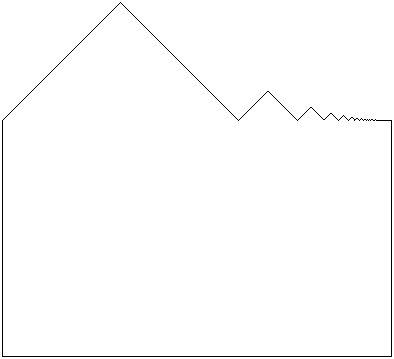
\includegraphics{\figdir/sawtooth-rectangle.pdf}
  \caption{A very excitable plane curve}
  \label{fig:excitable-plane-curve}
\end{figure}
Using a later result
(\cref{prop:replacing-by-same-endpoints}\footnote{This proposition
  basically just confirms that planar isotopy is legal even for
  general topological embeddings}), we can show that this is indeed a
tame knot. So, what happens if we try to ``thicken'' it to an
embedding of the torus? Here, we'll interpret ``thicken'' to mean
``find a simple rule to associate each point $p$ of this curve with a
2-disk $D_p \subseteq \RR^3$ such that $p$ is the center of $D_p$.''

If we try this with most polygonal knots $\msf K$, we can just think
of following an algorithm like the one below:
\begin{enumerate}[label=\arabic*)]\label{alg:tubular-neighborhood}
  \item Let $E$ denote the set of all the straight edges in $\fim{\msf
    K}{S^1}$. Let $r > 0$ be given by
    \[
    r = \min_{\substack{\msf E_1, \msf E_2 \in E \\ \msf E_1 \cap \msf
    E_2 = \varnothing}} d(\msf E_1, \msf E_2).
    \]
  \item For each vertex $x$ of $\msf K$ joining edges $\msf E_1$,
    $\msf E_2$, extend a line $\ell_x$ of length $2r$ through $x$ such
    that
    \begin{enumerate}
      \item $x$ is the midpoint of $\ell_x$, and
      \item In the plane $\aff\pn{\msf E_1, \msf E_2}$, $\ell_x$
        bisects $\angle \msf E_1\msf E_2$.
    \end{enumerate}
  \item Connect all the endpoints for consecutive $\ell_x$'s
    together in a way that ``follows'' the shape of $\msf K$
    (apologies for the lack of diagram here). This effectively gives
    us a ``ribbon'' tracing out the shape of $\msf K$.
  \item Finally, construct our embedded torus by ``sliding'' disks
    along the body of the knot, such that the boundary of each disk is
    always ``flush'' with the ribbon. This gives us an embedding of
    the torus.
\end{enumerate}
\begin{figure}[H]
  \centering
  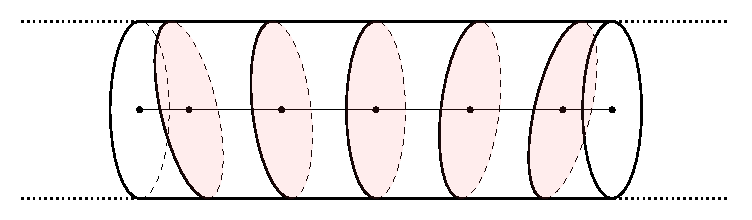
\includegraphics{\figdir/sliding-circle.pdf}
  \caption{An example of sliding the disks along.}
\end{figure}
This works out well-enough for most knots. Indeed, it seems
straightforward to extend this idea to all piecewise $C^1$ knots by
employing \emph{parallel curves:}\footnote{See
  \url{https://en.wikipedia.org/wiki/Parallel_curve}, for example.}
\begin{figure}[H]
  \centering
  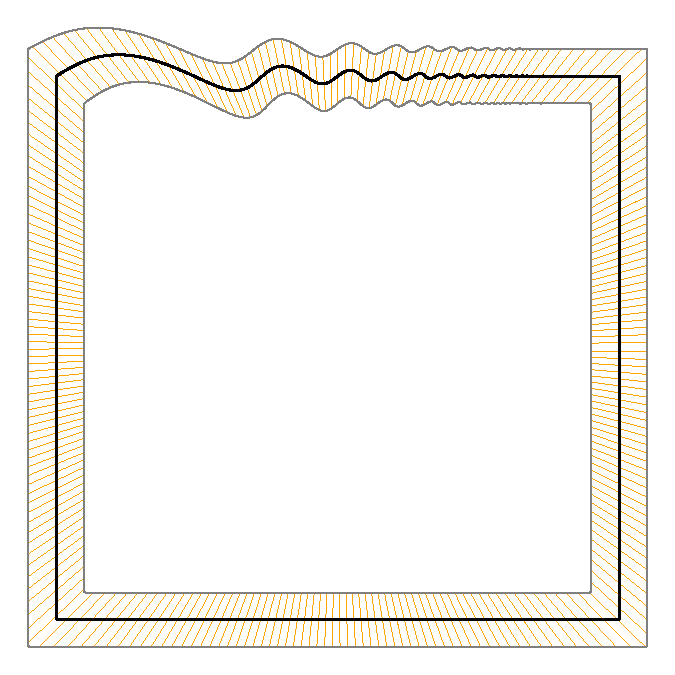
\includegraphics[scale=.7]{\figdir/countable-square-zigzag.pdf}
  \caption{An example for a piecewise $C^1$ knot. Note, this figure
    does not display \emph{actual} parallel curves, but rather just a
    slightly-shrunk and slightly-enlarged version of the square.}
\end{figure}
But again, it's not clear how to translate this to the context of our
knot in \cref{fig:excitable-plane-curve}, because we can't define $r$.
\begin{figure}[H]
  \centering
  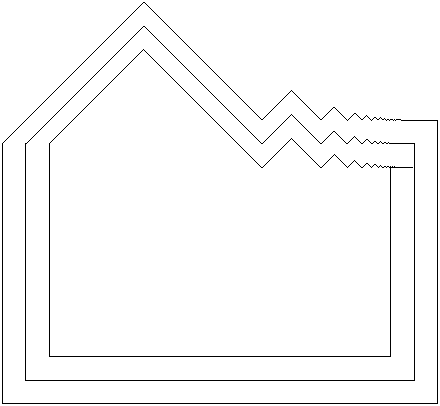
\includegraphics[scale=.9]{\figdir/sawtooth-rectangle-tube.pdf}
  \caption{An attempt to at a similar approach for the curve.}
\end{figure}
It doesn't work at the limit point of our sawtooth pattern. Fair
enough, the approach was quite naive. After some consternation, we
find that in this case, ``shrinking'' and ``enlarging'' the diagram
can get us what we want.
\begin{figure}[H]
  \centering
  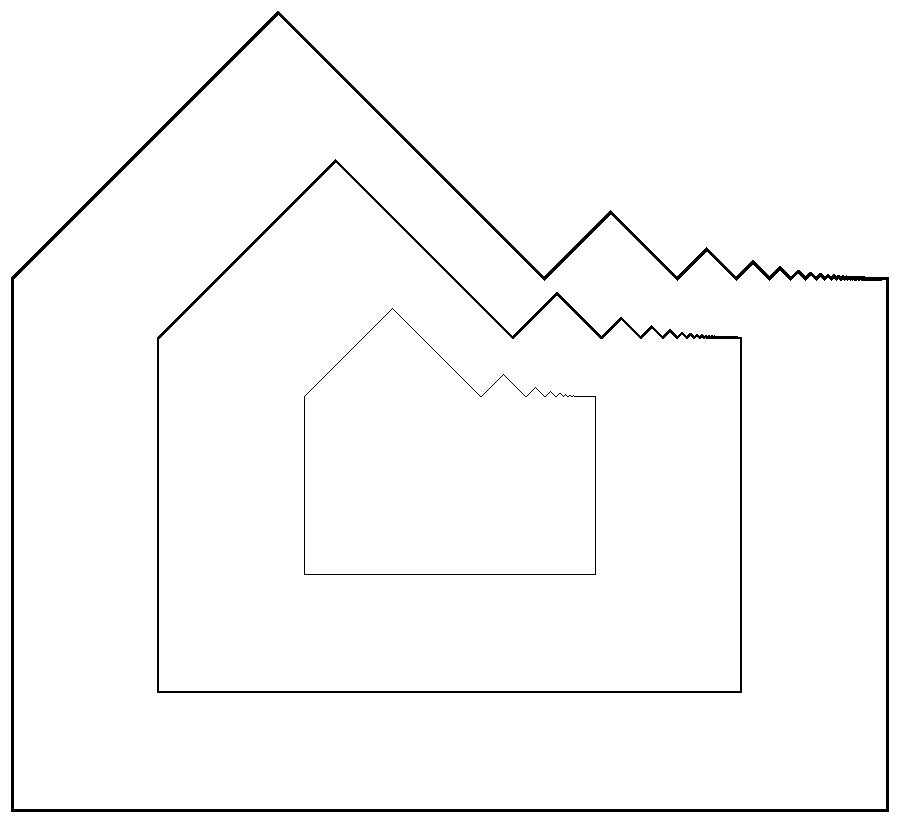
\includegraphics[scale=.5]{\figdir/sawtooth-shrink-shrunk.pdf}
  \caption{The desired embedding of the torus.}
\end{figure}
It's not immediately clear to us how to make this construction more
general, and we have not been able to find a proof or a more precise
statement of the claim. Hence, we propose a formal statement in the
below. We'll label it as a conjecture (even though it's almost surely
been proven before) because we have not worked out the full details
ourselves, due to time constraints. Our description uses the
definition of a \emph{lift}, which we state for purely comic effect.
\begin{definition}\label{def:lift}
  Let $C = (\mrm{ob}(C), \mrm{hom}(C))$ be a category. Let $X,Y,Z \in
  \mrm{ob}(C)$, and let $f \in \mrm{hom}(X,Y)$, $g \in
  \mrm{hom}(Z,Y)$, and $h \in \mrm{hom}(X,Z)$ such that $f = g \circ
  h$. Then we say that $h$ is a \emph{lift} of $f$, or that $f$
  \emph{factors through} $h$.
\end{definition}
\begin{figure}[H]
  \centering
  \begin{tikzpicture}
    \node (x) at (0,0) {$X$};
    \node (z) at (1.5,1.5) {$Z$};
    \node (y) at (1.5,0) {$Y$};

    \draw[->] (x) -- (y) node[midway, below] {$f$};
    \draw[->] (z) -- (y) node[midway, right] {$g$};
    \draw[->] (x) -- (z) node[midway, above left] {$h$};
  \end{tikzpicture}
  \caption{A commutative diagram for \cref{def:lift}}
\end{figure}
\begin{conjecture}\label{prop:lift-to-solid-torus}
  A knot $K : S^1 \into \RR^3$ is tame iff there exists an embedding
  $K_{\rm tor} : S^1\times \mbb{D}^2 \into \RR^3$ such that the
  embedding $\iota : S^1 \into S^1 \times \mbb{D}^2$ given by
  \[
    \iota(s) = (s, \mb 0)
  \]
  (where $\mb 0$ is the center of $\mbb{D}^2$)\footnote{Really, any
    point in $\pn{\mbb{D}^2}^\circ$ works.} satisfies $K = K_{\rm
  tor} \circ \iota$.
\end{conjecture}
\begin{figure}[H]
  \centering
  \begin{tikzpicture}
    \node (x) at (0,0) {$S^1$};
    \node (z) at (2,2) {$S^1 \times \mbb{D}^2$};
    \node (y) at (2,0) {$\RR^3$};

    \draw[->] (x) -- (y) node[midway, below] {$K$};
    \draw[->] (x) -- (z) node[midway, above left] {$L$};
    \draw[->] (z) -- (y) node[midway, right] {$K_{\rm tor}$};
  \end{tikzpicture}
  \caption{A commutative diagram for \cref{prop:lift-to-solid-torus}}
\end{figure}
It's worth mentioning that we have recently found a discussion of this
proposition in a MathOverflow post by user \cite{TubularNeighborhood};
however, a proof of the hard portion (existence of $K_{\rm tor}$
implies $K$ tame) was not included. We offer a tentative sketch of a
possible approach, but we offer no guarantees on correctness.
\begin{sproof}[Possible Sketch]
  Let $K : S^1 \into \RR^3$ be an embedding.
  \begin{iffproof}
  \item Suppose $K$ lifts to an embedding $K_{\rm tor} : S^1 \times
    \mbb{D}^2 \into \RR^3$ by the map $\iota : S^1 \into S^1 \times
    \mbb{D}^2$. Note, for all $s \in S^1$, the image $D_s =
    \fim{K_{\rm tor}}{s \times \mbb{D}^2} \subseteq\RR^3$ is
    homeomorphic to $\mbb{D}^2$, hence $\mrm{diam}(D_s) > 0$. Also
    observe that for all $t \in S^1$ with $t \neq s$, $t \not \in
    D_s$.\footnote{Even stronger, $D_t \cap D_s = \varnothing$}

    Show that in a non-trivially knotted region of $K$, the diameters
    $\mrm{diam}(D_s)$ are bounded by the distance between strands
    participating in a crossing. Then, suppose (to obtain a
    contradiction) that $K$ were wild. Show that the distance between
    crossing strands goes to $0$ as we approach the wild point, and
    obtain the contradiction.
  \item For the reverse proof, use the fact that $K$ is tame to obtain
    a homeomorphism $f : \RR^3 \to \RR^3$ such that $\msf K = f \circ
    K$ is polygonal. Construct the tubular neighborhood $N_{\rm tube}$
    of $\fim{\msf K}{S^1}$ using the
    \hyperlink{alg:tubular-neighborhood}{algorithm} described above
    (\cpageref{alg:tubular-neighborhood}). Note, since $f$ is a
    homeomorphism, $\fpre{f}{N_{\rm tube}}$ is homeomorphic to the
    torus $S^1 \times \mbb{D}^2$. Define $K_{\rm tor}$ in terms of
    $\fpre{f}{N_{\rm tube}}$, and show that it satisfies the desired
    properties.\renewcommand{\qedsymbol}{$\boxed{?}$}\qedhere
  \end{iffproof}
\end{sproof}
In any case: While this definition might have some theoretical
properties, it is hard to find a reference for, and seems to be easy
to accidentally misapply if care is not taken to be rigorous (e.g.,
again, we imagine most people employing this definition would guess
that \cref{fig:twists-perspective} is wild at first glance).

\begin{question}
  What does the torus in \cref{fig:twists-perspective} look like?
  We've managed to make some for earlier examples; e.g., an $xy$ plane
  projection of \cref{fig:3d-countable-reidemeister-i-plot} yields a
  picture that looks qualitatively similar to the following, hence we
  can draw a tubular neighborhood without too much trouble:
  \begin{figure}[H]
    \centering
    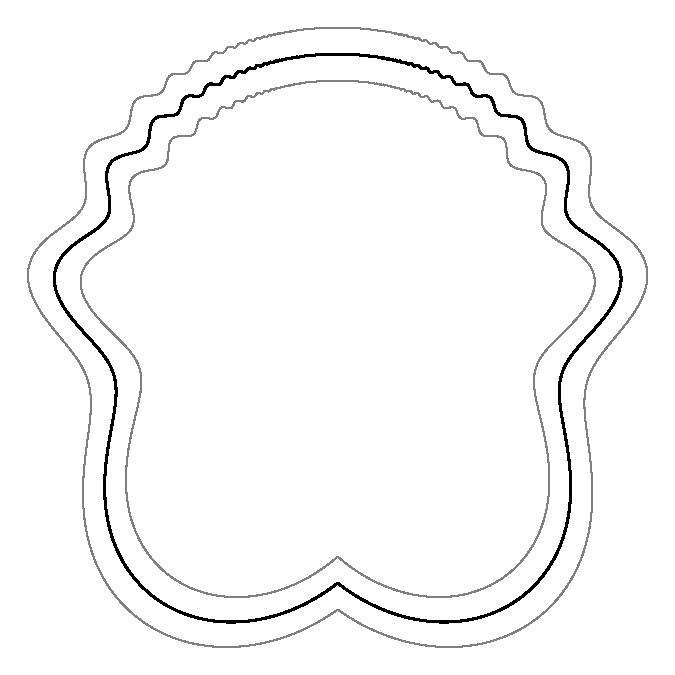
\includegraphics[scale=.7]{\figdir/smooth-countable-zigzag.pdf}
    \caption{A rough ``flavor'' for what the $xy$-plane projection of
      \cref{fig:3d-countable-reidemeister-i-plot} looks like. Note,
      this is actually a different (nicer-looking) function, but the
      idea is the same.}
  \end{figure}
  We'd be interested in seeing more plots of the associated embedded
  toruses for feral knots.
\end{question}


\section{Common Def. 4}
This section is very short: Given the abundance of examples of tame
knots with countably-many crossings that we have demonstrated, we
discourage the use of Common Definition \hyperlink{def:cdef4b}{4}. We
wonder whether the definition given there was supposed to be ``for
every tame knot $K : S^1 \into \RR^3$, there exists a projection $\pi
: \RR^3 \to \RR^2$ such that $\pi(K)$ has only finitely many
crossings.''

We are skeptical of this claim as well --- it's not obvious what there
is to stop us from taking 6 arcs shaped like the one in
\cref{fig:twists-perspective} and orienting them so that the ``core''
of each of the spirals (formally, the line normal to the plane in
\cref{fig:twists-top} passing through the center of the spiral) lies
along one of the $x,y$, or $z$ axes (each axis gets two spirals, one
pointing in the negative direction, the other pointing in the positive
direction). It seems that no projection of such a knot would yield
only finitely-many crossings, but we'd be willing to be surprised.

\section{Conclusion}
In this chapter, we've introduced several common definitions for
tameness/wildness/local flatness for knots, and established
correspondence (or lack thereof) with the definitions given in
\cite{Daverman}. We also gave a brief discussion of the differences
between the Topological, PL, $C^k$, and $C^\infty$ categories. The
remainder of this document will be concerned with building tools for
working hands-on with ambient isotopy in the Topological category. Our
goal is ultimately to lay the groundwork for characterizing ambient
isotopy between embeddings that can be represented by a countable
union of polygonal segments. To that end, we first turn our attention
to some machinery based in the tools of real analysis.





%%% Local Variables:
%%% TeX-master: "../../kobayashi-thesis"
%%% End:
